\section{Complementary analysis of the synthetic results}
\label{sec:posthoc}

The per-path predictions were recomputed from the frozen checkpoints
(maximum relative difference of $10^{-8}$ with respect to the reported MSE),
without retraining and without changing the protocol. Because the parameters
have different scales, each squared error is divided by the variance of the
parameter in the training set; the complementary result is the $R^2$ relative
to the trivial estimator that always predicts the prior mean.

\begin{table}[htbp]
\centering
\caption{Per-parameter $R^2$ relative to the prior mean, macro median
absolute error and MSE of the branching ratio on the synthetic test set.}
\label{tab:posthoc-r2}
\small
\begin{tabular}{lrrrrrr}
\toprule
Estimator & $\mu$ & $\alpha_{\mathrm{self}}$ & $\alpha_{\mathrm{cross}}$ & $\beta$ & Median AE & MSE of $g$\\
\midrule
Prior mean & $-$0.01 & 0.00 & $-$0.01 & 0.01 & 0.1908 & 0.0670\\
MLE & 0.24 & 0.90 & 0.90 & $-$15.64 & 0.0674 & 0.0023\\
LSTM (ensemble) & 0.84 & 0.82 & 0.81 & 0.65 & 0.0680 & 0.0017\\
Transformer (ensemble) & 0.84 & 0.74 & 0.73 & 0.61 & 0.0765 & 0.0019\\
\bottomrule
\end{tabular}
\end{table}

\begin{table}[htbp]
\centering
\caption{Paired comparison by path (mean standardized squared error over
the four parameters). Columns: median loss of A and of B, fraction of paths
in which A has the smaller error, and \emph{bootstrap} 95\% CI of the mean
difference A$-$B (negative favors A).}
\label{tab:posthoc-pareado}
\footnotesize
\begin{tabular}{llrrrr}
\toprule
A $\times$ B & Regime & Med.\ A & Med.\ B & A better & 95\% CI (A$-$B)\\
\midrule
LSTM $\times$ Transformer & all & 0.151 & 0.187 & 70.2\% & [$-$0.051, $-$0.047]\\
LSTM $\times$ Transformer & low $g$ & 0.112 & 0.131 & 61.1\% & [$-$0.021, $-$0.016]\\
LSTM $\times$ Transformer & intermediate $g$ & 0.127 & 0.164 & 72.8\% & [$-$0.045, $-$0.041]\\
LSTM $\times$ Transformer & near-critical $g$ & 0.237 & 0.304 & 76.7\% & [$-$0.089, $-$0.081]\\
\midrule
LSTM $\times$ MLE & all & 0.151 & 0.149 & 48.8\% & [$-$9.394, $-$0.809]\\
LSTM $\times$ MLE & low $g$ & 0.112 & 0.199 & 63.5\% & [$-$26.977, $-$2.225]\\
LSTM $\times$ MLE & intermediate $g$ & 0.127 & 0.100 & 40.1\% & [$-$0.040, $-$0.009]\\
LSTM $\times$ MLE & near-critical $g$ & 0.237 & 0.183 & 42.7\% & [$-$0.467, $-$0.277]\\
\midrule
Transformer $\times$ MLE & all & 0.187 & 0.149 & 43.5\% & [$-$9.376, $-$0.782]\\
Transformer $\times$ MLE & low $g$ & 0.131 & 0.199 & 59.4\% & [$-$27.686, $-$2.207]\\
Transformer $\times$ MLE & intermediate $g$ & 0.164 & 0.100 & 34.2\% & [0.002, 0.035]\\
Transformer $\times$ MLE & near-critical $g$ & 0.304 & 0.183 & 36.7\% & [$-$0.374, $-$0.195]\\
\bottomrule
\end{tabular}
\end{table}

First, the networks' advantage
over the MLE in aggregate MSE comes from a few paths: 94.4\% of the sum
of squared errors of the MLE's $\beta$ is concentrated in 1\% of the paths,
almost all of them in the low-$g$ regime. In all of the 300 worst paths, the
log-likelihood at the estimate exceeds that at the true parameter (median gain
of 2.80), and refitting 100 of them with 20 starts barely changes
the result. This is not a numerical failure: with weak excitation, $\beta$ is
weakly identified in 1,000 events. Second, on the typical path the MLE is as
good as the networks or better: its median loss is practically equal to the
LSTM's overall and lower in the intermediate and near-critical regimes. Third,
in the paired comparison the LSTM ensemble beats the Transformer ensemble in
every regime; across individual seeds, however, the difference is not
significant (Welch, $p=0.19$; Mann--Whitney, $p=0.056$),
because the LSTM showed two levels of convergence across seeds.

\begin{figure}[htbp]
\centering
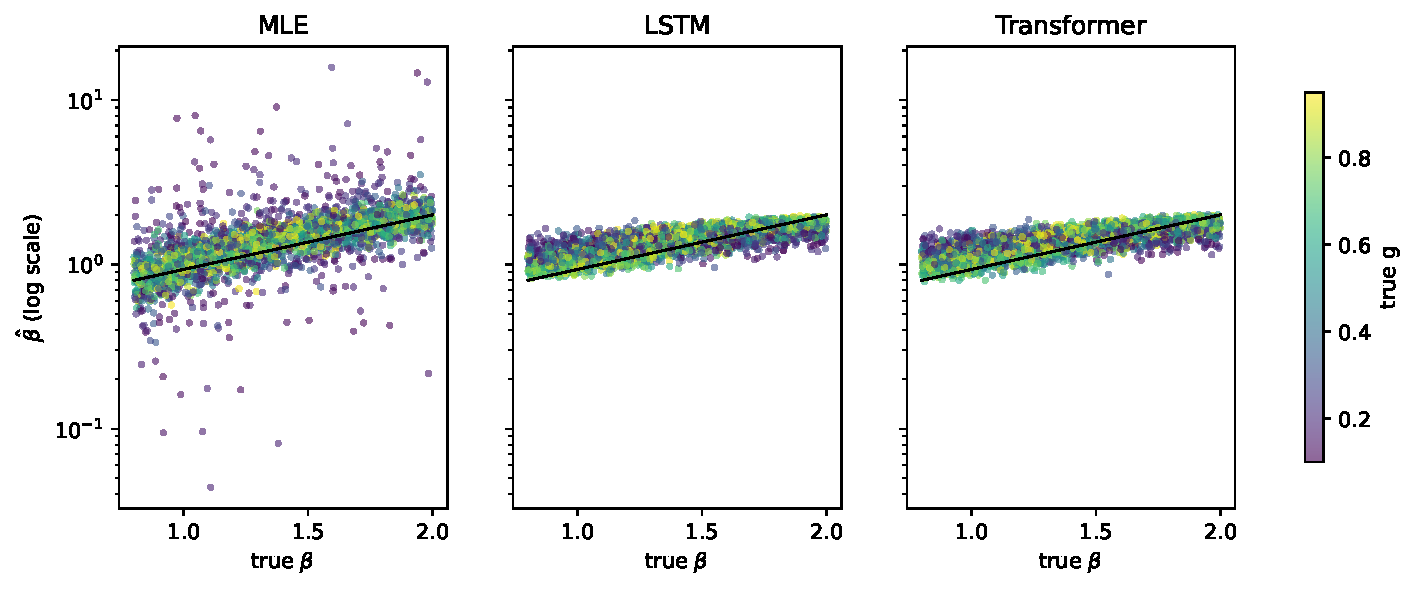
\includegraphics[width=0.95\linewidth]{../build/figures/posthoc_beta_verdadeiro_vs_estimado_en.pdf}
\caption{True versus estimated $\beta$ (3,000 test paths, logarithmic
scale). The networks shrink the estimates toward the center of the prior;
the MLE is unbiased over most of the domain but produces extreme values when
$g$ is low.}
\label{fig:posthoc-beta}
\end{figure}

\section{Empirical calibration and support of the synthetic prior}
\label{sec:calibracao}

The MLE was fitted on the 1,063 windows of 1,000 events
in the \texttt{calibration\_train} block (15 to 22 January 2024), the only
block authorized for calibration. The median $\beta$ was 2.71 (interquartile
range 2.21--3.14), above the upper limit of 2.0 used in training, and
$\alpha_{\mathrm{cross}}$ was below $10^{-3}$ in 89.4\% of the windows.
Only 15.4\% of the windows have $\beta$ inside the
prior, 0.4\% have the self-excited fraction
inside $[0.2,\,0.8]$, and 0.0\% satisfy all the ranges at once.
Because an estimator trained with quadratic loss approximates the posterior
mean under the training prior, the current networks cannot produce estimates
in this region; the empirical evaluation requires recalibrating the prior or
training on MLE labels from real windows.

\begin{figure}[htbp]
\centering
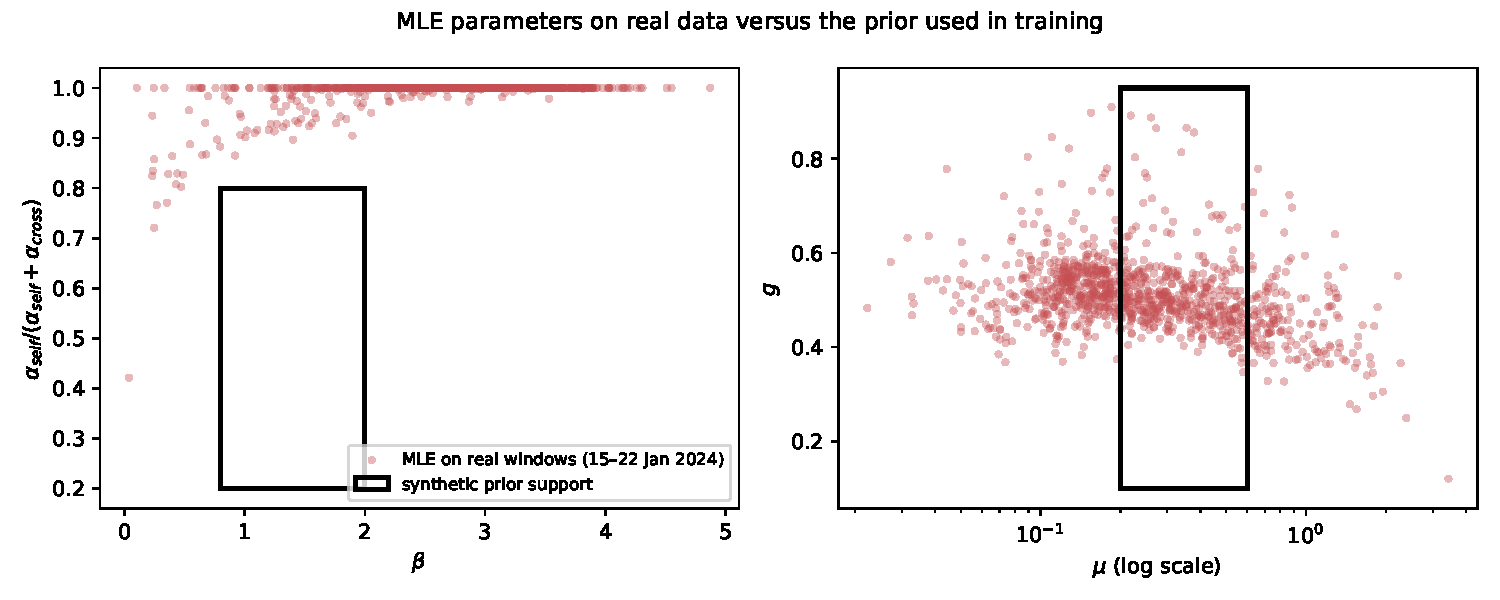
\includegraphics[width=0.95\linewidth]{../build/figures/posthoc_calibracao_vs_prior_en.pdf}
\caption{MLE estimates on the real calibration windows (points) and support
of the prior used to generate the training data (rectangles).}
\label{fig:calibracao-prior}
\end{figure}
